\documentclass[10pt,journal,compsoc]{IEEEtran}
\usepackage[lmargin=2cm, rmargin=2cm, top=1.5cm, bottom=2.5cm]{geometry}
\usepackage{longtable,multirow,booktabs}
\usepackage{mathrsfs} % para formato de letra
\usepackage[spanish,es-tabla]{babel}
\usepackage[utf8]{inputenc}
\usepackage[usenames]{color}
\usepackage[dvipsnames]{xcolor}
\usepackage{amsmath}
\usepackage{amsfonts}
\usepackage{amssymb}
\usepackage{cancel}
\usepackage{graphicx}
\usepackage{tikz}
\usepackage{float}
\usepackage{fancyhdr}
\usepackage[hidelinks]{hyperref} 
\graphicspath{imagenes}
\title{\bfseries \huge {Comandos Git} }
\author{
	\IEEEauthorblockN{Ezequiel Remus} 
	{|} \IEEEauthorblockA{
		Email: ezequielremus@gmail.com}
}

\oddsidemargin=-1cm

\renewcommand{\footrulewidth}{0,01cm}
\begin{document}
%\pagestyle{myheadings}
%TITULO
%modificar el formato del titulo
\maketitle
\newpage
\tableofcontents
%\newpage
\pagestyle{fancy}

\section{Iniciales}
Tener en cuenta que el doble guión debe ser consecutivo. 

Todos los comandos git comienzan con la palabra \textbf{git}.
\begin{enumerate}
\item \underline{\textit{\color{Blue}{git - -version}}}:\\
 Para conocer la version de git que tenemos.
\\

\item \underline{\textit{\color{Blue}{git config - -global user.name $"nombreDeUsuario"$}}}:\\
Lo primero que tenes que hacer después de instalar \textbf{git} es establecer tu nombre de usuario (y también después de correo electronico). Este comando sirve para establecer tu nombre de usuario.
\\

\item \underline{\textit{\color{Blue}{git config - -global user.email $"TuCorreo"$}}}:\\
Lo primero que tenes que hacer después de instalar \textbf{git} es establecer tu nombre de usuario y correo electronico. Este comando sirve para establecer tu correo.
\\

\textbf{Para mas información sobre el comando \textit{config} utilizar el comando: \color{Blue}{git - -help config}}


\end{enumerate}
%\newpage
\section{Repositorios}
Hay varias formas para trabajar con repositorios, en particular la que explico primero sin haber creado el repositorio desde git y otra habiendo primero creado un repositorio (hablando de repos propios, ya voy a explicar como laburar con repos en grupo). Yo en particular les recomiendo la segunda que es mas rapida (para mi).

Empecemos con la primera:

Creamos una carpeta, abrimos git bash y corremos el comando \textit{\color{Blue}{git init}}. Este comando lo que hace es decirle a git que inicie el seguimiento de la carpeta sobre la cual corrimos el comando. El comando crea una carpeta oculta llamada \textit{.git} donde git almacena su base de datos. Para ver esta carpeta, corremos el comando \textit{ls -a} este muestra todos los directorios, incluso los ocultos.

Luego, dentro de nuestra carpeta repositorio creamos el archivo \textbf{README.md}. Este archivo es un archivo de texto markdown el cual se utiliza para realizar la descripción del repositorio e inclusive dar una idea de lo que esta documentado. Dentro de este pondremos el titulo del repositorio de la siguiente forma 
$$ \# Nombre del Repositorio $$
Este va a ser nuestro titulo del \textit{README.md}.

Luego de guardar el \textit{README.md} corremos el comando \textit{\color{Blue}{git status}} que nos sirve para conocer en que estado esta el proyecto. Los estados pueden ser 2, todo rojo o todo verde. Si esta en rojo, significa que el archivo esta modificado y no esta subido (todabia esta en el working directory) a la base de datos git, en cambio si esta en verde significa que lo subis al \textit{staging area}, que es el area de preparacion. Para mover el archivo de la zona de trabajo a el area de preparacion se utiliza el comando \textit{\color{Blue}{git add .}}, al pasarle el punto le decis que suba todos los modificados, si queres solo subir uno de esos archivos le pasas el nombre del archivo con su extencion.

Luego, para que el archivo forme parte de nuestro historial de proyecto es necesario hacer un \textbf{commit}, esto es subir el archivo al directorio de git. el comando completo es: \textit{\color{Blue}{git commit -m $"$Comentario que represente al commit$"$}}. (\textit{\color{Red}{No necesariamente se abre vim para agregar el mensaje, que es lo que dice en el tutorial, lo mas rapido es hacer el comando como se los pase yo sin tener que entrar a ningun editor de texto para escribir el mensaje}}). 

Si corremos \textit{\color{Blue}{git status}} despues de este paso, vamos a ver que nos dice que ya esta todo listo para subir. Para poder subirlo tenemos que asociar la carpeta a un \textbf{repositorido github} para luego realizar  un \textbf{push}.

Para hacer un repositorio, entramos a nuestra cuenta github y nos logeamos.
 \begin{figure}[H]
  \begin{center}
	 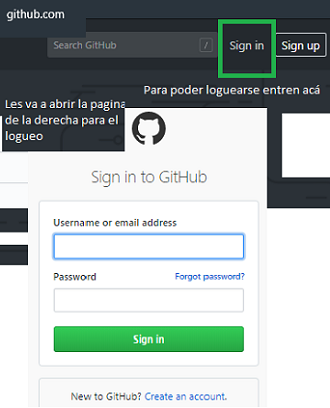
\includegraphics{figuras/logueo.png}
	 \centering
	 \renewcommand{\arraystretch}{1.3}
	 \caption{Pagina de github y logueo (aparecen en paginas diferentes)}
  \end{center}
\end{figure}

Despues del logueo van a la solapita con un signo de suma y apretan en \textbf{New Repository} 
 \begin{figure}[H]
  \begin{center}
	 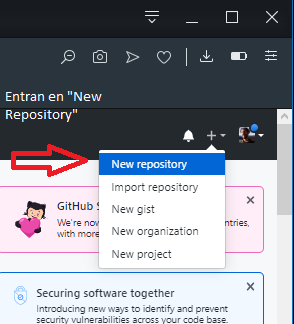
\includegraphics{figuras/repo.png}
	 \centering
	 \renewcommand{\arraystretch}{1.3}
	 \caption{Una vez logueados podemos crear un repo nuevo entrando a ese Boton}
  \end{center}
\end{figure}
Al entrar nos abre una ventana donde debemos tener en cuenta un par de cosas:

 Primero que nada, tenemos que ponerle un nombre si o si al repo (esto es poque sino no sabe a que corno apuntan los datos). 
 
 Por otra parte, \textit{yo prefiero en particular ahorrarme los pasos anteriores y crear primero el repositorio} con el \textit{README.md} desde la pagina (estamos hablando ya de la otra forma de las que les hable), te ahorras un par de comandos y es basicamente lo mismo.
 
  Los pasos anteriores sirven cuando ya tenes algo hecho y queres subirlo a un repo que ya existe o queres hacer un seguimiento de lo que fuiste haciendo a travez de los commits sin subirlo a un repositorio, en nuestro caso queremos trabajar con repos, por lo que les recomiendo primero crear el repositorio, clonar este en su pc (eso ya se los digo, es sencillo), poner los archivos que quieran subir y correr los comandos que venimos viendo de reconocimiento de estado, add y commit para poder subirlo y hacer el push directamente. Esto lo digo para que no se tengan que romper la cabeza para entrelazar la carpeta que creamos con las ramas del repositorio (origin y master) mediante comandos.
  
\begin{figure}[H]
  \begin{center}
	 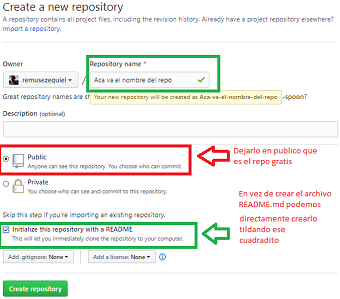
\includegraphics{figuras/crear.png}
	 \centering
	 \renewcommand{\arraystretch}{1.3}
	 \caption{Creando el repo}
  \end{center}
\end{figure}

Bueno, seguimos los pasos que aparecen en la \textit{Figura 3} y listo, ponemos \textbf{create repository} y se crea el repositorio. Yo cree uno para poner este pdf y despues voy a usarlo para poner apuntes, les dejo el link a este repositorio en las referencias por si lo quieren clonar cuando suba mas cosas y sino para que sepan que tambien pueden clonar repositorios de otros sin modificarles nada a los demas y asi poder leer las cosas de un repoistorio $x$ que les interese de una forma mas comodo.

\newpage
Bueno, siguiendo con esto de los repositorios, una ves creado el repositorio nos manda a la pagina del repo, que van a ver algo como esto:
\begin{figure}[H]
  \begin{center}
	 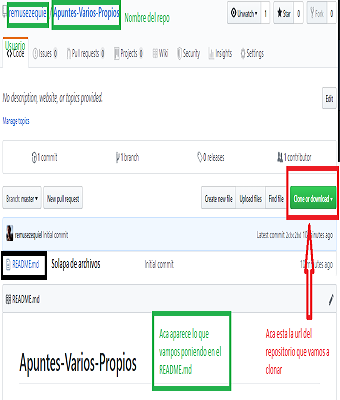
\includegraphics{figuras/repoNuevo.png}
	 \centering
	 \renewcommand{\arraystretch}{1.3}
	 \caption{Repo nuevo}
  \end{center}
\end{figure}
Ese es lo que se llama repositorio. Tenemos la parte de los archivos, donde ya de entrada vemos que aparece el archivo README.md, abajo de los archivos aparece lo que vamos escribiendo dentro del README (Si quieren no les ponen nada) este archivo es una guia sobre el repositorio, un resumen de lo que hay o muchas veces te explican como se usan o como se instalan los repositorios. Por ejemplo, estube viendo que el manejador de paquetes de Haskell \textit{Cabal} tiene su repositorio de github (dejo el link en referencias).
 
Ahora, para trabajar con este repositorio, tenemos que clonarlo en nuesto escritorio. Para eso, abrimos la terminal desde nuestro escritorio. tenemos que tener en cuenta, que si instalamos git en linux abrimos una terminal comun y nos corremos al Escritorio y ya esta, en windows, si siguieron los pasos del tutorial que puse en referencias para instalarlo e instalaron esa terminal que dice el pibe seria asi:

 \begin{figure}[H]
  \begin{center}
	 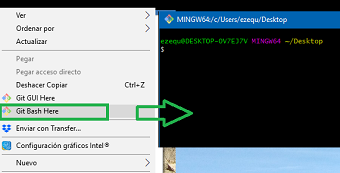
\includegraphics{figuras/consola.png}
	 \centering
	 \renewcommand{\arraystretch}{1.3}
	 \caption{Terminal desde windows}
  \end{center}
\end{figure}

Sino, si trabajan en linux y instalaron git con el comando \textit{\color{Green}{sudo apt-get install git}} abren una terminal de linux y corren los mismos comandos que voy a poner ahora, solo que clonan el repositorio que quieran clonar. En este caso, voy a clonar el repo que hice para este apunte. Para clonar el repositorio se utiliza el comando \textit{\color{Blue}{git clone urlDelRepositorio}}. El url lo sacan de la solapa \textbf{clone Repository} que esta en el repositorio, lo copian y lo pegan despues del comando git clone. Verifiquen que esten parados sobre el escritorio, sino se los va a clonar en otra ruta.

\begin{figure}[H]
  \begin{center}
	 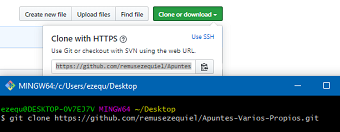
\includegraphics{figuras/clone.png}
	 \centering
	 \renewcommand{\arraystretch}{1.3}
	 \caption{Clonando el repositorio en el escritorio}
  \end{center}
\end{figure}

Vamos a ver que nos clona la carpeta en el escritorio con el nombre del repo. Abrimos la carpeta y vemos que el contenido es el mismo mas la carpeta oculta \textit{.git} de la que hablamos antes.


Ahora, lo que voy a hacer es poner la carpeta donde esta este pdf en el repositorio y voy a seguir los pasos de arriba:


 
 
 lo cual se hace con el comando \textit{\color{Blue}{git push origin master}}. Este comando lo voy a explicar mejor un poco mas adelante. Lo que es necesario entender hasta aca es que este comando lo sube a tu nube. Al ir a tu pagina en github, vas a ver que se renovo el repositorio de tu cuenta.
\\
\\
\\


%%%%%%%%%%%%%%%%%%%%%%%%%%%%%%%%%%%%%%%%%%%%%%%%%%%%%%%%%%%%%%%%%
\newpage
\begin{thebibliography}{1}
%
\bibitem{IEEEhowto:kopka}
 \emph{StackOverflow}, 
 Link: \textcolor{Red}{\url{https://stackoverflow.com}}
%
\bibitem{IEEEhowto:kopka}
 \emph{Link a un cursito de git basico}, 
 
 Link: \textcolor{Red}{\url{https://www.youtube.com/watch?v=m4wh8GhzcYg&list=PLmUnyBCRHkvUPkrsseI1SmMtYgfc-f8Kn&index=3}}
 %
 %
\bibitem{IEEEhowto:kopka}
Cuenta propia de github \emph{}.

 Link: \textcolor{Red}{\url{https://github.com/remusezequiel?tab=repositories}}
% 
%
\bibitem{IEEEhowto:kopka}
Repositorio de github donde se encuentra el codigo de este proyecto  \emph{}.

 Link: \textcolor{Red}{\url{https://github.com/remusezequiel/Apuntes-Varios-Propios}}
% 
%
\bibitem{IEEEhowto:kopka}
Repositorio de github donde se encuentra el proyecto Cabal  \emph{}.

 Link: \textcolor{Red}{\url{https://github.com/haskell/cabal}}


\end{thebibliography}

\end{document}